% Created 2017-09-19 Tue 18:00
% Intended LaTeX compiler: pdflatex
\documentclass[11pt]{article}
\usepackage[utf8]{inputenc}
\usepackage[T1]{fontenc}
\usepackage{graphicx}
\usepackage{grffile}
\usepackage{longtable}
\usepackage{wrapfig}
\usepackage{rotating}
\usepackage[normalem]{ulem}
\usepackage{amsmath}
\usepackage{textcomp}
\usepackage{amssymb}
\usepackage{capt-of}
\usepackage{hyperref}
\author{Francesco Ferraro, Diego Batista, Leonardo Martins}
\date{Setembro/2017}
\title{Linguagens, Automatos e Computação\\\medskip
\large Trabalho 1 - Linguagens Regulares}
\hypersetup{
 pdfauthor={Francesco Ferraro, Diego Batista, Leonardo Marques},
 pdftitle={Linguagens, Automatos e Computação},
 pdfkeywords={},
 pdfsubject={},
 pdfcreator={Emacs 25.1.2 (Org mode 9.0.10)}, 
 pdflang={English}}
\begin{document}

\maketitle
\begin{abstract}
Entrega formal do primeiro trabalho da disciplina de automatos na PUCRS.
\end{abstract}

\section{Questão 1 - Cadeias}
\label{sec:org6854e37}
\subsection{Terminam por bcb}
\label{sec:orgce1b984}
\begin{figure}[htbp]
\centering
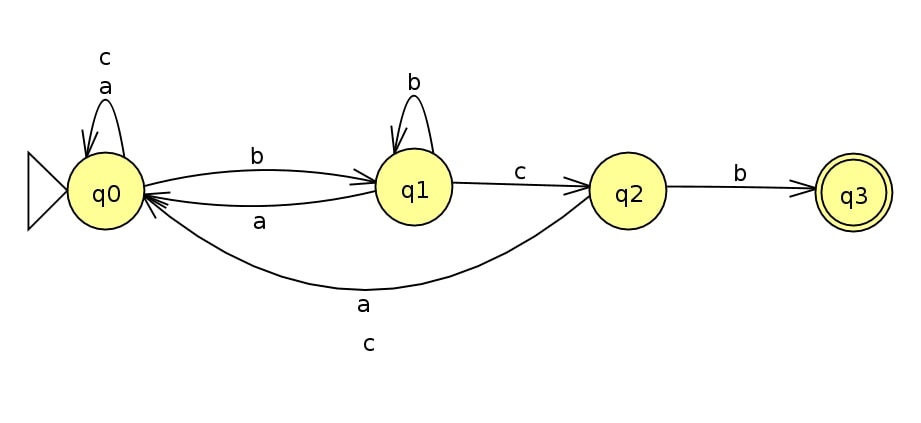
\includegraphics[width=.9\linewidth]{./q1/a/q1a.jpg}
\caption{\label{fig:org666ee09}
Esse é um autômato determinístico}
\end{figure}

\begin{center}
\begin{tabular}{ll}
Input & Result\\
\hline
abcb & Accept\\
bcbb & Reject\\
cbcb & Accept\\
bcbaaa & Reject\\
aaaaa & Reject\\
\end{tabular}
\end{center}

\subsection{Terminam por no máximo dois b´s}
\label{sec:orge75716f}
\begin{figure}[htbp]
\centering
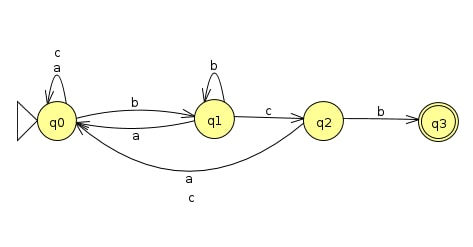
\includegraphics[width=.9\linewidth]{./q1/b/q1b.jpg}
\caption{\label{fig:orga8a9744}
Esse é um autômato determinístico}
\end{figure}

\begin{center}
\begin{tabular}{ll}
Input & Result\\
\hline
b & Reject\\
a & Reject\\
c & Reject\\
bb & Reject\\
aba & Reject\\
ac & Reject\\
ab & Reject\\
bc & Reject\\
ba & Reject\\
\end{tabular}
\end{center}

\pagebreak
\subsection{Não terminam por dois bs consecutivos}
\label{sec:org99ff2b8}
\begin{figure}[htbp]
\centering
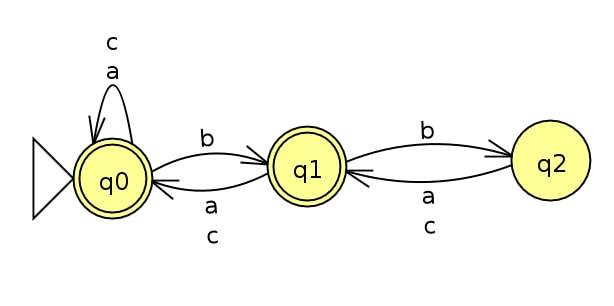
\includegraphics[width=.9\linewidth]{./q1/c/q1c.jpg}
\caption{\label{fig:orgb375888}
Esse é um autômato determinístico}
\end{figure}

\begin{center}
\begin{tabular}{ll}
Input & Result\\
\hline
aa & Accept\\
bb & Reject\\
cc & Accept\\
c & Accept\\
a & Accept\\
b & Accept\\
aacbac & Accept\\
abcabc & Reject\\
\end{tabular}
\end{center}
\pagebreak
\subsection{Iniciam por a e terminam com c}
\label{sec:orgc6bebc2}
\begin{figure}[htbp]
\centering
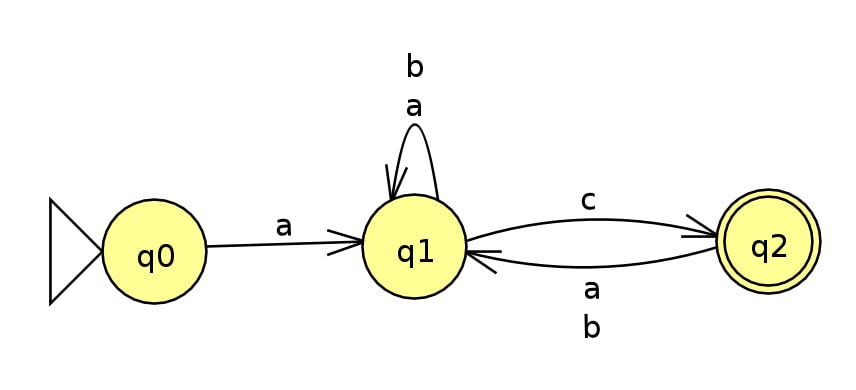
\includegraphics[width=.9\linewidth]{./q1/d/q1d.jpg}
\caption{\label{fig:org710fe77}
Esse é um autômato determinístico}
\end{figure}

\begin{center}
\begin{tabular}{ll}
Input & Result\\
\hline
a & Reject\\
b & Reject\\
c & Reject\\
ac & Accept\\
abcbc & Accept\\
acac & Accept\\
abcbb & Reject\\
\end{tabular}
\end{center}
\pagebreak
\subsection{Iniciam e terminam pelo mesmo símbolo}
\label{sec:org9356ea2}
\begin{figure}[htbp]
\centering
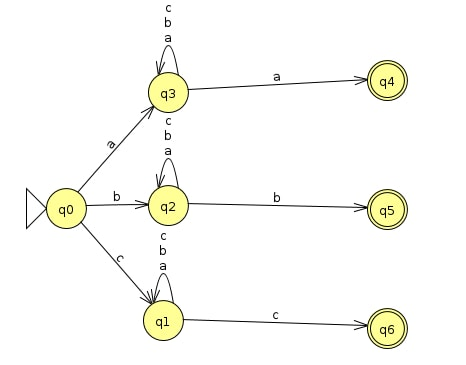
\includegraphics[width=.9\linewidth]{./q1/e/q1e.jpg}
\caption{\label{fig:org6c94205}
Esse é um autômato determinístico}
\end{figure}

\begin{center}
\begin{tabular}{ll}
Input & Result\\
\hline
aa & Accept\\
bb & Accept\\
cc & Accept\\
ac & Reject\\
ab & Reject\\
bbaa & Reject\\
bba & Reject\\
\end{tabular}
\end{center}
\pagebreak
\subsection{Iniciam e terminam por símbolos diferentes}
\label{sec:org1f27122}

\begin{figure}[htbp]
\centering
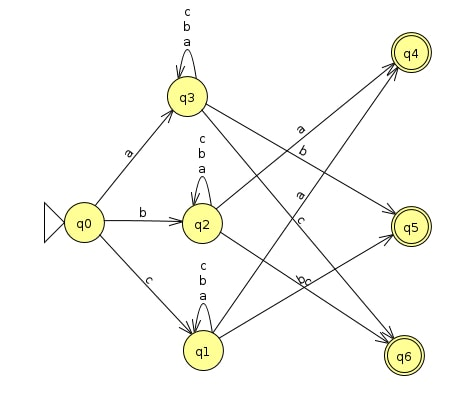
\includegraphics[width=.9\linewidth]{./q1/f/q1f.jpg}
\caption{\label{fig:org67f1480}
Esse é um autômato não determinístico}
\end{figure}

\begin{center}
\begin{tabular}{ll}
Input & Result\\
\hline
aa & Reject\\
bb & Reject\\
cc & Reject\\
ac & Accept\\
ab & Accept\\
bbaa & Accept\\
bba & Accept\\
abcbcba & Reject\\
\end{tabular}
\end{center}

\pagebreak
\subsection{Número ímpar de b’s}
\label{sec:org334c150}
\begin{figure}[htbp]
\centering
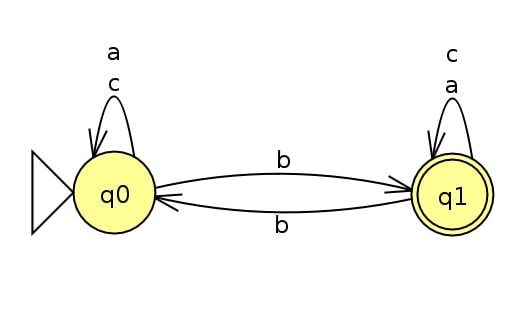
\includegraphics[width=.9\linewidth]{./q1/g/q1g.jpg}
\caption{\label{fig:org841d2b6}
Esse é um autômato determinístico}
\end{figure}

\begin{center}
\begin{tabular}{ll}
Input & Result\\
\hline
aa & Reject\\
bb & Reject\\
cb & Accept\\
ac & Reject\\
ab & Accept\\
bbaa & Reject\\
bba & Reject\\
abcbcba & Accept\\
b & Accept\\
\end{tabular}
\end{center}
\pagebreak
\subsection{Não possuam dois símbolos iguais adjacentes}
\label{sec:orgac60c58}
\begin{figure}[htbp]
\centering
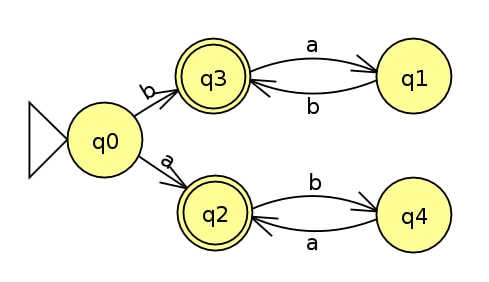
\includegraphics[width=.9\linewidth]{./q1/h/q1h.jpg}
\caption{\label{fig:org419664d}
Esse é um autômato determinístico}
\end{figure}

\begin{center}
\begin{tabular}{ll}
Input & Result\\
\hline
a & Accept\\
b & Accept\\
aa & Reject\\
bb & Reject\\
abba & Reject\\
baab & Reject\\
abababa & Accept\\
baba & Reject\\
\end{tabular}
\end{center}
\pagebreak

\section{Questão 2 - Expressões Regulares}
\label{sec:org47235f9}
\subsection{Terminam por 101}
\label{sec:orgf7dddd2}

\begin{quote}
(0+1)*(101)
\end{quote}

\subsection{Iniciam por 1 e terminam com 0}
\label{sec:org72abd86}

\begin{quote}
1(1+0)*0 
\end{quote}

\subsection{Iniciam e terminam pelo mesmo símbolo}
\label{sec:orgd8b3031}

\begin{quote}
1(1+0)*1 + 0(1+0)*0 
\end{quote}

\subsection{Iniciam e terminam por símbolos diferentes}
\label{sec:org952d3ca}

\begin{quote}
1(1+0)*0 + 0(1+0)*1 
\end{quote}

\subsection{Terminam por no máximo dois 0´s}
\label{sec:orgd66519e}
\begin{quote}
((0+1)* + (100))+ ((0+1)* + (10)) +((0+1)* + (1)*)
\end{quote}
\pagebreak
\section{Questão 3 - 10n1}
\label{sec:orgea1570a}
\subsection{Automato}
\label{sec:org4a57c10}
A figura \ref{fig:org779decc} reponde essa questão. 

\begin{figure}[htbp]
\centering
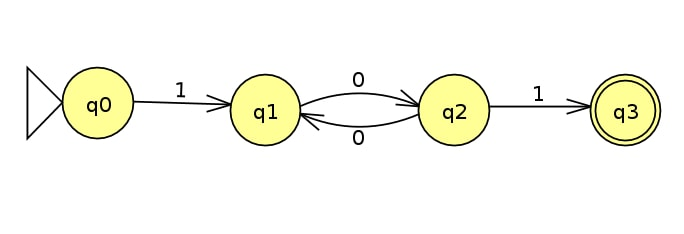
\includegraphics[width=.9\linewidth]{./q3/q3.jpg}
\caption{\label{fig:org779decc}
Esse é um autômato determinístico}
\end{figure}

\begin{center}
\begin{tabular}{rl}
Input & Result\\
\hline
0 & Reject\\
01 & Reject\\
1 & Reject\\
101 & Accept\\
1001 & Reject\\
10001 & Accept\\
100001 & Reject\\
1000001 & Accept\\
10000001 & Reject\\
\end{tabular}
\end{center}
\subsection{Expressão regular}
\label{sec:org13b3bdc}

\textbf{10+(00)*+1} 
\pagebreak
\section{{\bfseries\sffamily TODO} Questão 4 - AFND -> AFD}
\label{sec:orgb81e8e2}
Aqui vai uma super resolução.
\begin{figure}[htbp]
\centering
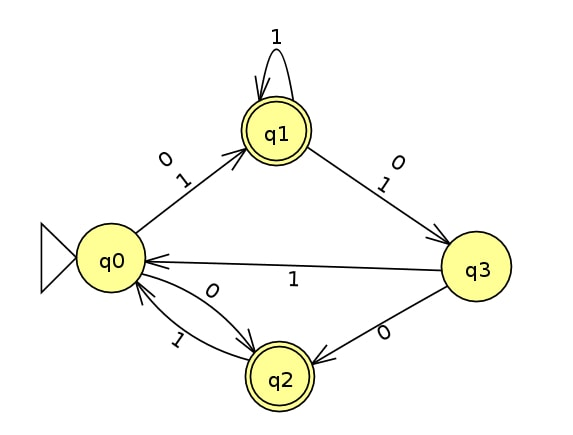
\includegraphics[width=.9\linewidth]{./q4/q4.jpg}
\caption{\label{fig:org909fda7}
Esse é um autômato determinístico}
\end{figure}
\pagebreak
\section{Questão 5  - V ou F}
\label{sec:orgd4e3a61}
\subsection{Falso}
\label{sec:org2726acf}
Uma vez que consumidas todas as entradas o AFND acaba com a execução ainda que a transição do vazia para o mesmo estado ocorra.  O fato de que o estado anterior a ela ser o mesmo que o posterior não faz o autômato entrar em loop.
\subsection{Verdadeira}
\label{sec:org9ce3c42}
\subsection{Falso}
\label{sec:org1745221}
Um ADF sem ao menos 1 estado final reconhece só a linguagem vazia.
\subsection{Falsa}
\label{sec:orgebd3a12}
Por definição um AFD e AFND tem igual poder de reconhecimento

\pagebreak
\section{Questão 6 - Estacionamento}
\label{sec:orge5f19b3}
Resposta é a figura \ref{fig:org5fd4825}.
\begin{figure}[htbp]
\centering
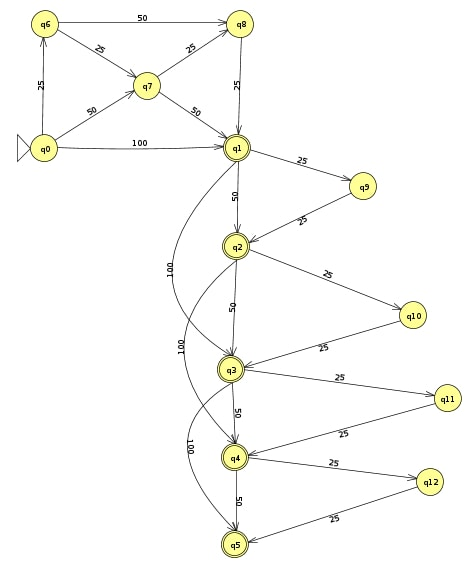
\includegraphics[width=.9\linewidth]{./q6/estacionamento.jpg}
\caption{\label{fig:org5fd4825}
Autômato de uma parquímetro}
\end{figure}
\pagebreak
\section{Questão 7 - Sinaleira}
\label{sec:org0e51221}
\subsection{Analisando os semáforos paralelamente.}
\label{sec:org423dfdb}

Resposta é a figura \ref{fig:orgac52818}.
\begin{figure}[htbp]
\centering
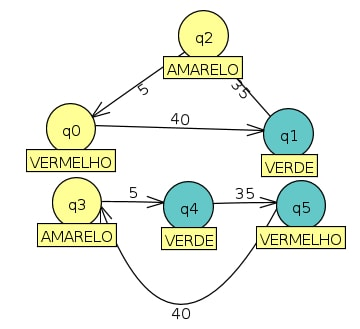
\includegraphics[width=.9\linewidth]{./q7/paralelo.jpg}
\caption{\label{fig:orgac52818}
Autômato em paralelo}
\end{figure}

\subsection{Analisando os semáforos simultaneamente.}
\label{sec:org95ad0ae}

Resposta é a figura \ref{fig:org75ec515}.
\begin{figure}[htbp]
\centering
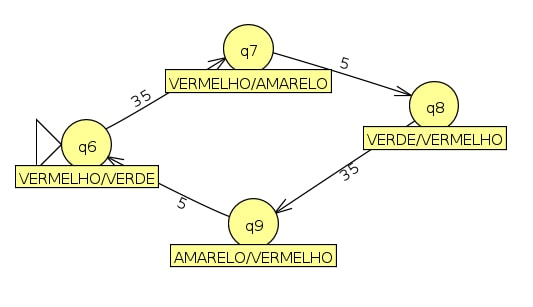
\includegraphics[width=.9\linewidth]{./q7/simultaneo.jpg}
\caption{\label{fig:org75ec515}
Autômato simultâneo}
\end{figure}
\end{document}
